\section{Methodology}
\label{sec:implementation}

\subsection{GTZAN Dataset}

GTZAN contains 1000 clips (10 genres, 100 clips each)~\cite{tzanetakis2002gtzan}. One file (\texttt{jazz.00054.wav}) is corrupted, so the usable dataset size is 999.

I used both modalities:
\begin{itemize}
\item \textbf{Image path}: precomputed spectrogram images.
\item \textbf{Audio path}: waveform clips converted to MFCC-based sequences.
\end{itemize}

\begin{figure}[t]
	\centering
	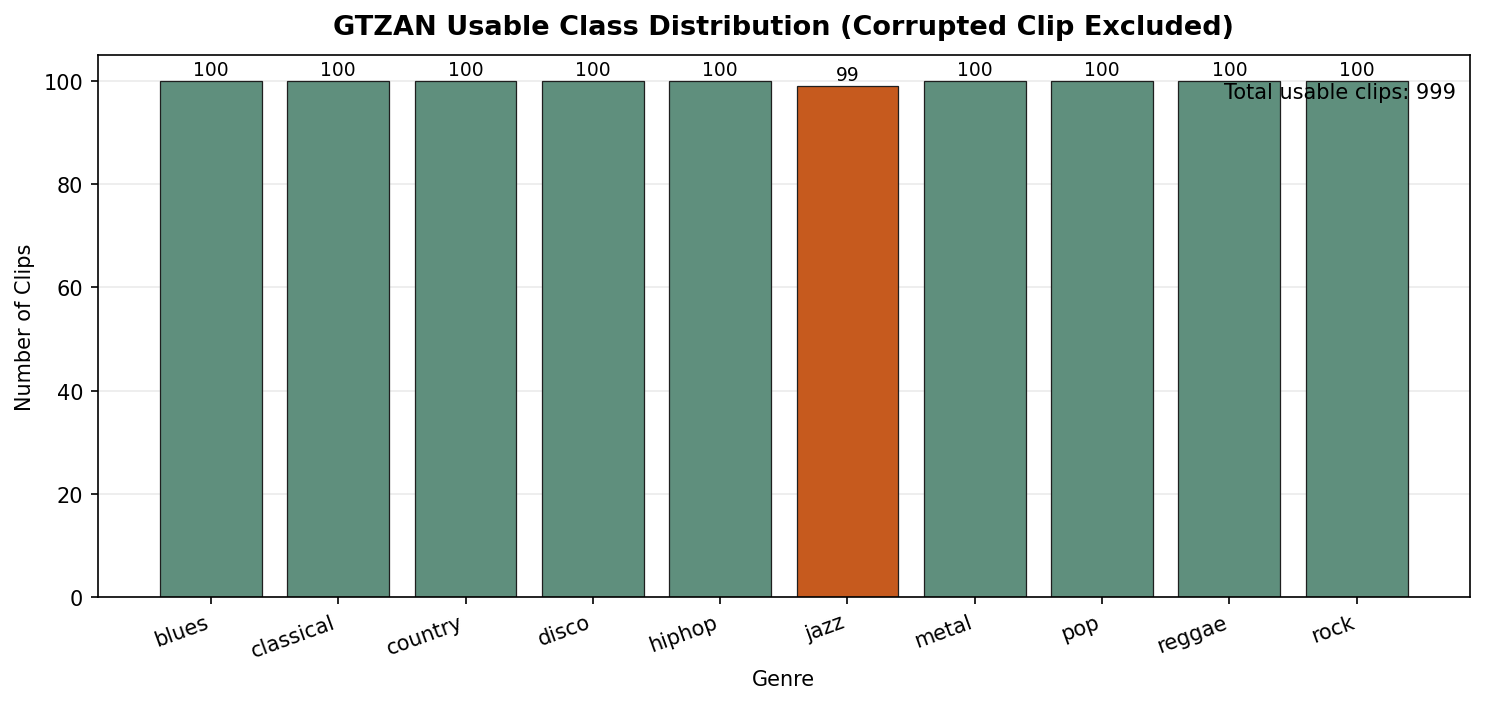
\includegraphics[width=\linewidth]{figures/gtzan_dataset_overview.png}
	\caption{GTZAN class balance and distribution used in this project (999 usable clips).}
	\label{fig:dataset-overview}
\end{figure}

\subsection{Data Split and Preprocessing}

I created one shared stratified split for every model: 70\% train, 20\% validation, 10\% test. Using one split keeps the comparison fair.

For image models (Net1--Net4), each spectrogram is resized to $180\times180$, converted to tensor, and normalized.

For audio models (Net5--Net6), each clip is resampled to 22050~Hz and converted to 80-dim features (40 MFCC + 40 delta). Sequences are padded/truncated to 320 frames.

\subsection{Neural Network Architectures}

\begin{itemize}
\item \textbf{Net1}: fully connected image baseline.
\item \textbf{Net2}: CNN baseline.
\item \textbf{Net3}: CNN + batch normalization.
\item \textbf{Net4}: Net3 architecture trained with RMSProp.
\item \textbf{Net5}: bidirectional LSTM on MFCC sequences.
\item \textbf{Net6}: Net5 with GAN-augmented training data.
\end{itemize}

\subsection{Training and Evaluation Setup}

All models are implemented in PyTorch~\cite{paszke2019pytorch}. Image models were trained up to 100 epochs with best-validation checkpoint loading. Sequence models used early stopping and gradient clipping for stable training.

Cross-entropy loss was used for classification. Adam/AdamW was used in most models, while Net4 used RMSProp by design. Net6 used weighted handling of synthetic samples during training.

The same test split was used for all six models. I report accuracy and macro-F1, then compare model groups (4 image models, 2 audio models, all 6 together) and summarize the main error pattern.